% !TEX TS-program = xelatex
% !TEX encoding = UTF-8 Unicode

% \documentclass[AutoFakeBold]{LZUThesis}
\documentclass[AutoFakeBold]{LZUThesis}
\setCJKfamilyfont{XST}{新宋体}

\begin{document}

\title{{深度Koopman算子辅助的}{非线性系统强化学习研究}}

\entitle{{ Deep Koopman Operator Assisted }{ Reinforcement Learning of Nonlinear System }}

\author{{\CJKfamily{XST} \zihao{3} 许忞欢}}
\major{电子信息科学与工程}
\advisor{赵东东}
\college{信息科学与工程学院}
\grade{2020级}

\maketitle

%==============================%
% ↓ ↓ ↓ 诚信说明页 授权说明书
%==============================%

% 1. 可以调整签字的宽度,现在是40
% 2. 去掉raisebox的相关注释(注意上下大括号对应),可以改变-5那个数字调整签名和横线的上下位置

% 你的签名,signature.pdf 改为你的签名文件名,
\mysignature{
    % \raisebox{-5pt}{
    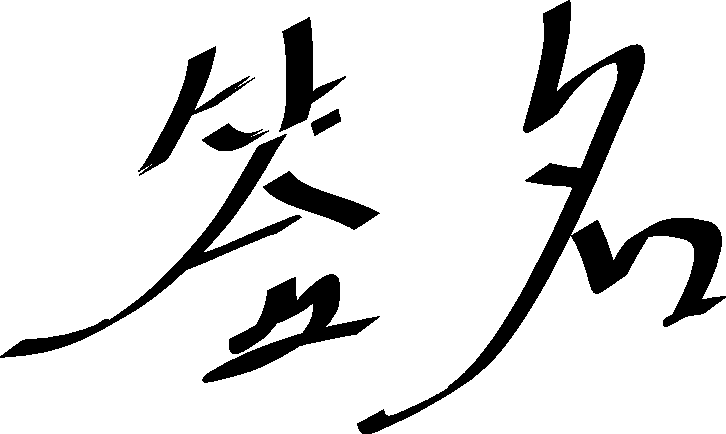
\includegraphics[width=40pt]{signature.pdf}
    % }
}
% 你手写的日期,signature.pdf 改为你的手写的日期文件名
\mytime{
    % \raisebox{-5pt}{
    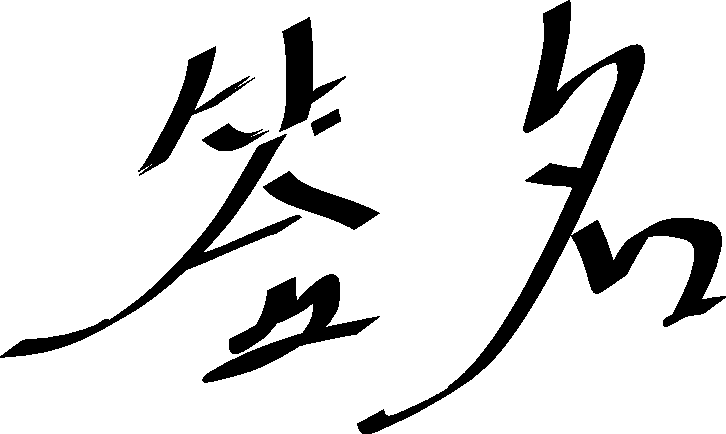
\includegraphics[width=40pt]{signature.pdf}
    % }
}
% 老师的手写签名,signature.pdf 改为老师的手写签名文件名
\supervisorsignature{
    % \raisebox{-5pt}{
    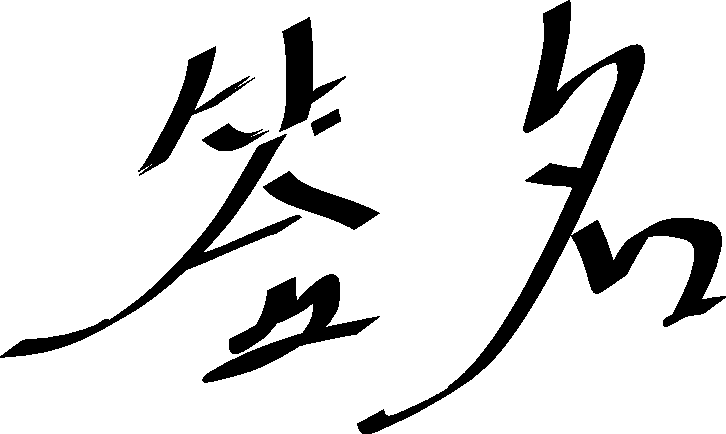
\includegraphics[width=40pt]{signature.pdf}
    % }
}
% 老师手写的时间,signature.pdf 改为老师的手写的日期文件名
\teachertime{
    % \raisebox{-5pSt}{
    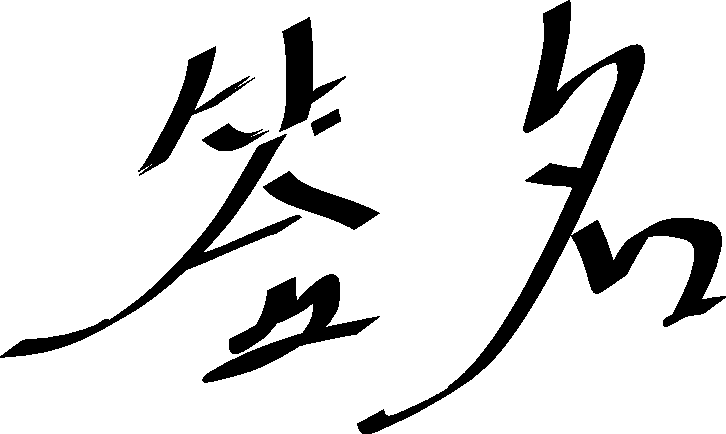
\includegraphics[width=40pt]{signature.pdf}
    % }
}
% 老师手写的成绩
\recommendedgrade{
    % \raisebox{-5pt}{
    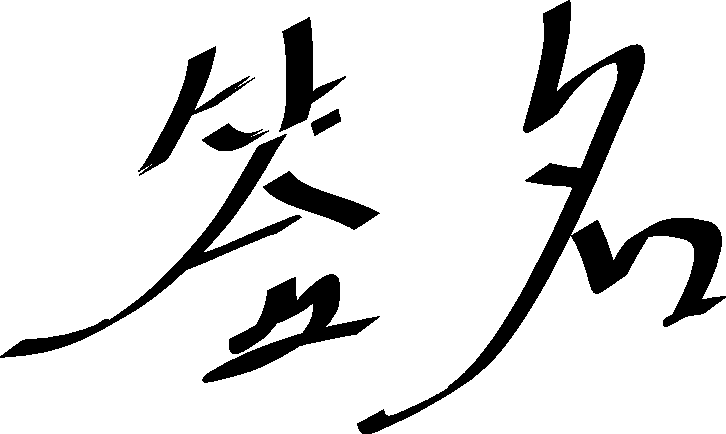
\includegraphics[width=40pt]{signature.pdf}
    % }
}

\makestatement

%==============================%
% ↑ ↑ ↑ 诚信说明页 授权说明书
%==============================%


%=====%
%论文(设计)成绩:注意2007的模板要求,成绩页在最后,2021要求成绩页在摘要前面
%=====%

% 下面这些注释掉可以去掉成绩、评语什么的
% \supervisorcomment{好好好}
%
%
% \committeecomment{优秀}
%
% \finalgrade{100}
% 上面这些注释掉可以去掉成绩、评语什么的


\frontmatter



%中文摘要
\ZhAbstract{这是测试的参考文献。}
{Koopman算子理论,深度神经网络,强化学习}

%英文摘要
\EnAbstract{My Abstract}
{Koopman Operator Theory, Deep Neural Network, Reinforcement Learning}

%生成目录
\tableofcontents
% 下面这个包含图表目录
% \customcontent


% 部分同学需要专业术语注释表,* 表示不加入目录
% \chapter*{专业术语注释表}
% \begin{longtable}{lll}
%   \caption*{缩略词说明}\\
%   SS & Spread Spectrum & 扩展频谱 \\
%   PAPR & Peak to Average Power Ratio & 峰均比\\
%   DCSK & Differential Chaos Shift Keying &差分混移位键控\\
%   dasd & fdhfudw eqwrqw fasfasfs fewev wqfwefew &\tabincell{l}{太长了\\换行一下}\\
% \end{longtable}


%文章主体
\mainmatter

\chapter{\texorpdfstring{绪 \quad 论}{绪论}}

\section{研究背景及意义}
% 当前,非线性系统控制领域正处于快速发展的阶段。
% 研究者们在多个方面进行着深入探索,以解决实际问题并推动技术进步。
% 首先,建模方法方面,我们见证了物理模型、数据驱动模型和混合模型等多种方法的发展。
% 这些方法基于不同的原理,旨在更准确地描述系统的动态特性。
%
% Koopman算子理论作为一种描述动力学系统演化的数学工具,
% 将系统的动态演化提升到无穷维函数空间中进行线性演化。
% Koopman算子的引入可以为强化学习非线性系统控制方法提供了一个新的思路。
%
% 深度学习具有潜力实现可扩展和数据驱动的架构,用于发现和表示Koopman特征函数,
% 提供了对强非线性系统进行升维并线性表示的可能性。
% 这样的做法能够对现代动力学系统中的两个关键挑战起缓解的作用:
% 尽管神经网络(Neural Network)几十年来一直都被用于建模动力学系统和其他的物理学过程,
% 但最近在使用深度神经网络(Deep Neural Network, DNN)学习Koopman嵌入方面取得了巨大进展。
% 在最近的研究中,DNN被证明在挑战性问题上比其他主流方法具有更灵活的特点并且更具有准确性。
%
% DNN表示的Koopman特征函数,
% 即使对于高维和强非线性系统也保持可解释和简洁。
% 特别是,许多动力学系统表现出连续的特征值谱,
% 这使得使用现有的DNN或Koopman表示进行低维表示变得困难。
% 对于具有连续谱的系统,可以利用增强型网络来对嵌入系统上的线性动态进行参数化,
% 避免在谐波特征函数中进行无限渐近展开。
% 因此,得到的网络保持简洁,并且少量关键的特征函数是可解释的。
% 如上的深度学习方法在Koopman算子理论上的应用,
% 展示了该方法的强大性,
% 同时在经典动力学系统方面保持直观性。
%
% 强化学习(RL)是机器学习和控制理论交叉领域中快速发展的领域,
% 其中智能体学习如何与环境交互以达到最大化回报的目标。
% 而Koopman算子和深度学习的引入,
% 可以使强化学习更好的完成非线性系统的控制任务。



% \section{国内外研究现状}

\subsection{深度强化学习}
强化学习是一个快速发展的领域,处于机器学习和控制理论的交叉点,
其中智能体学习在复杂的环境进行交互以实现目标\cite{Brunton_book_2019}。
深度强化学习 最近被证明能够在几个具有挑战性的
任务\cite{van_hasselt_deep_2016, sanghi_introduction_2021}中
实现人类水平或超人类的表现,
包括玩视频游戏\cite{mnih_human-level_2015, vinyals_grandmaster_2019}和
策略游戏\cite{silver_mastering_2016, silver_mastering_2017, silver_general_2018}。
深度强化学习也越来越多地用于科学和工程应用,
包括用于药物发现\cite{popova_deep_2018}、
机器人操作\cite{gu_deep_2017}、
自动驾驶\cite{sallab_deep_2017}
和无人机竞速\cite{kaufmann_champion-level_2023}、
流体流动控制\cite{gazzola_reinforcement_2014, colabrese_flow_2017, 
verma_efficient_2018, novati_controlled_2019, 
fan_reinforcement_2020}和聚变控制\cite{degrave_magnetic_2022}。

尽管取得了上述进展,深度强化学习解决方案通常需要巨大的计算资源来训练和泛化,
并且它们通常缺乏在许多应用中至关重要的可解释性。
许多强化学习策略背后的算法与优化和最优控制理论\cite{Brunton_book_2019}中的
贝尔曼方程(Bellman Equation)及其连续形式
汉密尔顿-雅可比-贝尔曼(Hamilton-Jacob-Bellman)方程密切相关。
然而,求解这些方程对于高维非线性系统来说变得棘手,这通常可以使用深度学习来缓解。
在\cite{karl}的工作中,通过Koopman算子的新应用改写贝尔曼方程,
在无限维函数空间上将非线性动态系统重塑为线性方程组。

\subsection{Koopman算子理论}
Koopman算子\cite{koopman_hamiltonian_1931, 
koopman_dynamical_1932, mezic_comparison_2004}
在缓解未知动力学下非线性控制的这种困难方面表现出巨大的潜力。
作为一种数据驱动的方法,Koopman算子可以用最小二乘法自动学习系统模型。
此外,Koopman算子可以将非线性动力学映射到嵌入空间中的线性系统。
并且嵌入式线性系统已准备好通过LQR\cite{bemporad_explicit_2002}和MPC\cite{fernandez-camacho_robust_1995}等线性方法进行控制。
尽管如此,选择嵌入函数以保持预测质量仍然是一项艰巨的任务。
最近的方法侧重于用深度神经网络\cite{mainuddin_detecting_2023}学习嵌入函数,然后应用线性控制方法\cite{han_deep_2020}。
在\cite{dkn}中,提出了一个端到端的深度学习框架,
将Koopman嵌入函数和Koopman算子一起学习,缓解了上述困难。

\section{本文主要工作}
本文主要研究了如何使用改进的最大熵强化学习算法实现对于非线性动力学系统的最优控制。
本文利用了最大熵强化学习算法构建了非线性系统最优学习问题,并通过引入深度Koopman算子,
对问题中涉及的强化学习对于强非线性的适应性问题进行改善,最后利用实现的深度Koopman算子辅助
的最大熵强化学习算法对强非线性系统进行最优控制。

第一章为绪论,主要分析了使用深度Koopman算子和最大熵强化学习的研究背景和意义,并介绍了本文的结构。

第二章为基础知识,首先介绍了Koopman算子理论的基本概念,并阐述了高阶升维系统的得到和与原系统的数学关系;
然后介绍本文使用的基础强化学习框架,并着重介绍了本文强化学习和其他算法的核心结合点:马尔可夫决策过程和贝尔曼方程;
最后提及简单的神经网络架构,为本文中特殊函数参数化做铺垫。

第三章介绍了如何通过数据驱动的方式的到受控的、动作相关的Koopman算子,并介绍如何将其引入马尔可夫决策过程,
进而改进价值估计,使得强化学习方式更好地解决非线性系统控制问题。

第四章介绍如何通过深度学习方式得到非线性动作相关的Koopman算子,并将其融入第三章得到的算法框架中,并通过实验的方式
证明改进的有效性。最后,提出当前算法的问题,给出未来展望。


\chapter{基础知识}
在本章中,首先讨论一下有关的背景理论与算法。
介绍一下Koopman算子理论(Koopman Operator Theory),
并讨论Koopman算子对于重塑强化学习(Reinforcement Learning)
中使用的马尔可夫决策过程(Markov Decision Process)的重要作用。
同时,对于Koopman算子理论与深度神经网络(Deep Neural Network)之间的关联。

\section{Koopman算子理论}
系统的强非线性是数据驱动建模和控制领域的核心问题之一,包括基于现代强化学习框架所做的工作。
Koopman算子理论\cite{}为上述问题提出了一种解决方案。
在该理论中,非线性系统动力学可以在提升到无限维度希尔伯特空间时变为线性系统,
并可以通过一组新的基底对于该线性系统进行观测。
升维工作已被证明对于线性化和简化某些具有挑战性的问题具有显著效果,这与机器学习领域中其他的类似努力相一致。

\subsection{Koopman算子与非线性系统演化}
我们应该采用不同的形式对不同类型的系统中系统状态$x$进行描述。
假设系统为确定性自治系统,我可以采用下面的方式,将一个离散动力系统描述为
\begin{equation}
  \dot{x} = F(x)
\end{equation}
其中,$\Dot{x}$表示下一个时刻的系统状态;或者,采取不同的方式,将一个连续动力系统描述为
\begin{equation}
  \frac{\mathrm{d}}{\mathrm{d}t} x(t) = f(x(t))
\end{equation}
而在处理实际问题是,我们通常考虑的是离散动力系统。
所以我们就可以将连续系统通过流映射算子(Flow Map Operator)归纳为一个离散系统,系统演化如下
\begin{equation}
  x(t + \tau) = F_\tau(x(t)) = x(t) + \int^{t + \tau}_t f(x(s)) \mathrm{d}s
\end{equation}

Koopman算子提供了解决非线性系统控制问题的一个新的着眼点。
在形式上,我们考虑一个实值向量测量函数$g: M \to \mathbb{R}$,且都由无限维希尔伯特空间的元素组成,其中$M$是一个流形。
通常,这个流形被认为是$L^\infty(X), \ X \subset \mathbb{R}^d$。
一般情况下,函数$g$可被称为观测函数。
Koopman算子理论中指出,Koopman算子$\mathcal{K}$和Koopman生成器$\mathcal{L}$
都是作用于上述观测函数$g$的无限维线性算子,在确定性系统中,有
\begin{subequations}
  \begin{align}
    \mathcal{K}g &= g \circ F \\
    \mathcal{L}g &= f \cdot \nabla g
  \end{align}
\end{subequations}
Koopman生成器$\mathcal{L}$和Koopman算子有如下的关系
\begin{equation}
  \mathcal{L} g = \lim_{t \to 0} \frac{\mathcal{K}g - g}{t} = \lim_{t \to 0} \frac{g \circ F - g}{t}
\end{equation}

Koopman算子理论可以更广泛地应用于任何马尔可夫过程,但本文以随机性连续时间系统为例,此时,Koopman算子的定义如下:
\begin{align*}
  \mathcal{K} g &= \mathbb{E} (g(X) | X_0 = \cdot) \\
  \mathcal{L} g &= \lim_{t \to 0} \frac{\mathcal{K} g - g}{t}
\end{align*}

Koopman算子将测量函数$g$沿着路径$x$向前演化如下:
\begin{equation}
  \mathcal{K}_\tau g(x_t) := g(F_\tau(x_t)) = g(x_{t + \tau})
\end{equation}
其中$F$代表着系统的演化规律。更一般的,在随机自治系统中,$\mathcal{K}$被如下定义为条件预测算子:
\begin{equation}
  \mathcal{K} g(x_t) = \mathbb{E}\left[g(X_{t + \tau}) | X_t = x_t\right]
  \label{Linear_Predictor_K}
\end{equation}
在上述离散系统算子中,普遍使用$\mathcal{K} := \mathcal{K}_1$,在本文中也照此用法。

% 值得注意的是,如上文所述,Koopman算子$\mathcal{K}$是一种作用于观测函数$g$的无限维线性算子,这意味着在由观测两系统的演化规律也将是线性的;

\subsection{Koopman算子本征函数}
上文提出,可观测函数$g$的观测,都存在于无限维的希尔伯特空间中(被称作观测空间),
被如Koopman算子$\mathcal{K}$等无限维的算子推动沿着给定非线性动力学系统演化。
因此不难发现,我们可以应用Koopman算子理论研究,将对于非线性系统的研究,通过观测空间状态线性演化实现。

同时,由于难以捕捉无限维希尔伯特空间中所有可观测函数的演化,所以应该试图识别随着非线性系统动力学而线性演化的关键观测函数,
Koopman算子的本征函数就可以作为一组特殊的观测函数[cite]:
\begin{equation}
  \mathcal{K} \Phi (x_k) = \lambda \Phi(x_k) = \Phi(x_{k + 1})
\end{equation}
此时,本征函数就会成为观测空间的一组基底,由此,数学上,观测函数应当表示为这组基底的线性组合,如下:
\begin{equation}
  g(x) = \sum_{i = 1}^n a_i \Phi_i(x)
\end{equation}
此时,观测空间可被称为状态字典空间,同时,空间的基底可被称为字典函数

当前,从数据中挖掘信息并获得Koopman本征函数是现代动力学系统研究的主流方法,被称为数据驱动(Data-Driven)的Koopman算子。
由此,我们可以通过数据驱动的方式得到Koopman算子的本征函数,以得到非线性系统在高维空间中的全局线性表示。

此外,Koopman算子已经被广泛运用于受控系统。
在受控确定性离散时间系统中,我们有:
\begin{equation}
  x' = F(x, u)
\end{equation}
在受控连续时间系统中:
\begin{equation}
  \frac{\mathrm{d}}{\mathrm{d}t} x = f(x(t), u(t))
\end{equation}

如果考虑到$u_{k + 1} = u_k$的控制输入,
我们可以将等式 (\ref{Linear_Predictor_K}) 修改为:
\begin{equation}
  g(x_{k + 1}, u_{k + 1}) = \mathcal{K} g(x_k, u_k)
  \label{Linear_Predictor_with_Control}
\end{equation}
其中$x \in \mathbb{R}^n, u \in \mathbb{R}^m$,
且$g : \mathbb{R}^{n + m} \mapsto \mathbb{R}^d$。




\section{强化学习}

\subsection{马尔可夫决策过程与贝尔曼方程}
马尔可夫决策过程是具有马尔可夫性质的随机过程。

随机过程是指研究对象是随时间演变的随机现象,在随机过程中,随机现象在某一时刻$t$的取值是一个向量随机变量,可以用$S_t$表示,所有可能的状态组成状态空间$\mathcal{S}$。
我们将已知所有历史状态$( S_1,\dots,S_t )$时,某一时刻$t$的状态$S_t$发生的概率用$P( S_{t + 1} | S_1,\dots,S_t )$表示。
而马尔可夫性质则表示,已知当前时刻状态$S_t$时,下一时刻状态$S_{t + 1}$仅与$S_t$有关,用$P( S_{t + 1} | S_t)$表示。而从前一状态经过随机进入下一状态的过程被称为状态转移。

在下文中,我们假设存在一个无限时域的马尔可夫决策过程。我们假设代理跟随随机策略$\pi(u | x)$,表示在已知状态$x$的情况下,采取某个特定动作$u$的可能性。
由此,在离散时间系统中,状态价值函数定义为:
\begin{equation}
  V^{\pi}(x) = \mathbb{E} \left[ \sum_{k = 0}^{\infty} \gamma^k r(x_k, u_k) |
  \pi, x_0 = x \right]
\end{equation}
其中,$r(x_k, u_k)$ 表示智能体得到的奖励;
$\gamma \in [0, 1]$ 表示折扣率,用于避免在无限时域时无限大的奖励。

在这里我们强调强化学习与控制领域的结合,所以本文中考虑使用线性二次最优控制问题。
线性二次最优控制是十分经典的控制领域问题,其中线性代表研究的系统动态可以用一组线性微分方程表示,
而其成本为二次泛函。
形式上,我们考虑有限时间长度,离散时间的LQR,假设离散时间线性系统:
$$
x_{k + 1} = A x_k + B u_k
$$
其性能指标为:
\begin{equation}
  c(x_k, u_k) = x_k^T Q x_k + u_k^T R u_k
\end{equation}
将系统线性二次性能指标的相反数作为智能体探索时的奖励:
\begin{equation}
  r(x_k, u_k) = - c(x_k, u_k)
\end{equation}
并改写贝尔曼方程可以得到:
\begin{equation}
  V^{\pi}(x) = \mathbb{E} \left[ \sum_{k = 0}^{\infty} - \gamma^k c(x_k, u_k) | \pi, x_0 = x \right]
\end{equation}

\subsection{演员-评委强化学习算法}
演员-评论家(Actor-Critic)强化学习算法是一种结合价值学习和策略学习的强化学习算法,
下面分三步介绍Actor-Critic强化学习算法。

首先介绍策略学习,在策略学习中,评价一个策略的方法是评估策略在环境中获得的回报的期望,此时目标函数为:
\begin{equation}
  J(\theta) = \mathbb{E}_S\left[ V_\pi (S) \right]
\end{equation}
其中,$V_\pi$代表状态价值函数,可以看到在这个目标函数中,
求得了状态价值函数有关状态的期望,所以只涉及到策略$\pi$的信息。
同时易知,这个目标函数该期望越大,表明该策略越好。

注意,在本文中,对于强化学习的研究只涉及深度强化学习,所以在这里使用深度神经网络的方式对策略网络进行测试。
所以,问题转化为如下的一个最大化问题:
\begin{equation}
  \max_{\theta} J(\theta)
\end{equation}
很明显,我们只需要使用梯度上升的方式迭代策略网络。
参数更新如下:
\begin{equation}
  \theta_{new} = \theta_{old} + \beta \cdot \nabla_\theta J(\theta_{now})
\end{equation}
其中,$\beta$代表学习率,是需要调整的超参数,
梯度的具体表达式如下:
\begin{equation}
  \nabla_\theta J(\theta_{now}) \triangleq \frac{\partial J(\theta)}{\partial \theta}
\end{equation}
以上算法被称为策略梯度

在策略学习中,我们想要得到的是当前策略能得到的价值函数,表示如下:
\begin{equation}
  V^\pi(s_t) = \mathbb{E} \left[ \sum_{k = t}^{N}
  \gamma^{k - t} \cdot r_k \right]
\end{equation}
在深度强化学习中,我们通过深度神经网络对价值进行近似,算法上,应该使得上述价值网络逼近真实价值函数。
一般使用时间差分(Temporal Differencial)算法来更新价值函数,根据贝尔曼方程:
\begin{equation}
  V^{\pi}(s_t) = \mathbb{E} \left[ r_t + \gamma V^\pi(s_{t + 1}) \right]
\end{equation}
等式左边为价值函数处于时间步$t$时对于价值的估计,等式右边是对于左边的一个无偏估计,
其中包含的$r_t$项使得等式右边比左边更加精确,所以应当使得价值网络逼近等式右边的值。
参数更新如下:
\begin{equation}
  Q^{new}(s_t, a_t) \leftarrow (1 - \alpha) Q^{now}(s_t, a_t) 
  + \alpha [ r_t + \gamma Q^{now}(s_{t + 1}, a_{t + 1}) ]
\end{equation}

最后,通过交替执行策略优化和价值优化,可以使得两者的性能逐渐同步提升。
策略网络可以获得更好的状态价值,价值网络可以实现更好的价值估计。
最后取用策略网络作为最优控制的策略函数就可以完成Actor-Critic算法在最优控制问题上的应用。

\section{神经网络}
本文中将使用简单的神经网络对函数进行近似,在本节中将对于神经网络进行一些简单的介绍。
\subsection{简单架构}
神经网络架构和人类大脑中的神经细胞很像,
它们相互连接组成了一个复杂的神经细胞网络状的结合体,
可以发送电信号来交换信息。
而人工神经网络由人工神经细胞构成,
以相似的结构组合起来,共同合作以求解决实际问题。

基本的神经网络有三层\cite{noauthor_-_nodate}:
\begin{enumerate}
  \item 输入层:数据通过输入层经过处理进入网络;
  \item 隐藏层:从输入层或其他隐藏层获取数据并计算输出;
  \item 输出层:给出最后的结果,一般具有非线性;
\end{enumerate}

具有上述基本层的网络叫全连接层,下面介绍全连接层\cite{noauthor__2024}:
令输入向量$x \in \mathbb{R}^d$,神经网络的一个层把$x$映射为$x' \in \mathbb{R}^{d'}$。全连接层定义如下:
\begin{equation}
  x' = \sigma(z), \qquad z = W x + b
\end{equation}
其中,权重矩阵 $W \in \mathbb{R}^{d' \times d}$和
偏置向量$b \in \mathbb{R}^{d'}$是该层的参数,需要从数据中学习;
$\sigma(\cdot)$是激活函数,比如softmax函数、sigmoid函数,ReLU(Rectified Linear Unit)函数。
最常用的激活函数是ReLU。定义如下:
\begin{equation}
  \mathrm{ReLU}(z) = [(z_1)_+, (z_2)_+, \cdots, (z_{d'})_+,]^T
\end{equation}
上面的$[z_i]_+ = \max(z_i, 0)$。我们称上面的结构为全连接层(Fully Connected Layer)。
如果把全连接层当作基本部件,然后像搭积木一样搭建一个全连接神经网络,
也叫多层感知机(Multi-Layer Perceptron, MLP)

\subsection{反向传播}
线性模型和神经网络的训练都可以描述成一个优化问题,
设全连接层的权重参数为$\omega^{(1)}, \cdots, \omega^{(l)}$
我们希望求解下面这样的一个优化问题\cite{noauthor__2024}:
\begin{equation}
  \min_{\omega^{(1)}, \cdots, \omega^{(l)}} L(\omega^{(1)}, \cdots, \omega^{(l)})
\end{equation}
其中$L$表示损失函数。
对于这样一个无约束的最小化问题,最常使用的方法是梯度下降(Gradent Descent, GD)和随机梯度下降(Stochastic Gradient Descent, SGD),本节主要介绍使用SGD求解最小化问题。

假设目标函数可以写成$n$连加的形式:
\begin{equation}
  L(\omega^{(1)}, \cdots, \omega^{(l)}) = \frac1n \sum_{j = 1}^{n}
  F_j (\omega^{(1)}, \cdots, \omega^{(l)})
\end{equation}
函数$F_j$隐含第$j$个训练样本$(x_j, y_j)$。
每次从集合$\{ 1,2,\cdots,n \}$中随机抽取一个数,记作$j$。
当前的参数只为$\omega_{now}^{(1)}, \cdots, \omega_{now}^{(j)}$,
计算此处的梯度,SGD算法的迭代过程为
\begin{equation}
  \omega_{new}^{(i)} \leftarrow \omega_{now}^{(i)} - 
  \alpha \cdot \underbrace{
  \nabla{\omega^{(i)}} F_j \left( \omega_{now}^{(1)}, 
\cdots, \omega_{now}^{(l)} \right)}_\text{随机梯度},
  \quad \forall i = 1, \cdots, l.
\end{equation}

下面我们介绍反向传播(Backpropagation,BP),以全连接神经网络为例,简单介绍反向传播的原理。
全连接神经网络(忽略偏移量$b$)定义如下:
\begin{align*}
  x^{(1)} &= \sigma_1 (W^{(1)} x^{(0)}), \\
  x^{(2)} &= \sigma_2 (W^{(2)} x^{(1)}), \\
  &\vdots                                \\
  x^{(l)} &= \sigma_l (W^{(l)} x^{(l - 1)}),
\end{align*}
神经网络的输出$x^{(l)}$是神经网络做出的预测。设向量$y$为真实标签,函数$H$为交叉熵,实数$z$为损失函数:
\begin{equation}
  z = H(y, x^{(l)})
\end{equation}
要做梯度下降更新参数$W^{(1)}, \cdots, W^{(l)}$,我们需要计算损失函数$z$关于每一个变量的梯度:
\begin{equation}
  \frac{\partial z}{\partial W^{(1)}}, \frac{\partial z}{\partial W^{(2)}}, 
  \cdots, \frac{\partial z}{\partial W^{(l)}}
\end{equation}

现在可以用链式法则做反向传播,计算损失函数$z$关于神经网络参数的梯度。
具体地,首先求出梯度$\frac{\partial z}{\partial x^{(l)}}$。
然后做循环,从$i = l, \cdots, 1$,依次执行如下操作:
根据链式法则可得损失函数$z$关于参数$W^{(i)}$的梯度:
\begin{equation}
  \frac{\partial z}{\partial W^{(i)}} = \frac{\partial x^{(i)}}{\partial W^{(i)}} 
  \cdot \frac{\partial z}{\partial x^{(i)}}
\end{equation}
此梯度用于更新参数$W^{(i)}$。
根据链式法则可得损失函数$z$关于参数$x^{(i - 1)}$的梯度:
\begin{equation}
  \frac{\partial z}{\partial x^{(i - 1)}} = \frac{\partial x^{(i)}}{\partial x^{(i - 1)}} 
  \cdot \frac{\partial z}{\partial x^{(i)}}
\end{equation}
这个梯度被传播到下面一层(即第$i - 1$层),继续循环。

综上所述,只要知道损失函数$z$关于$x^{(i)}$的梯度,就能求出$z$关于$W^{(i)}$和$x^{(i - 1)}$的梯度。

\chapter{Koopman算子辅助的最大熵强化学习}

贝尔曼方程及其连续形式汉密尔顿-雅可比-贝尔方程
在强化学习和控制理论中普遍存在。
然而,这些方程对于具有高维状态和非线性的系统来说,很快就变得难以处理。
本章将讨论数据驱动的Koopman算子与马尔可夫决策过程之间的联系,
并介绍借由此开发的两种新的强化学习算法来解决上述的问题。

技术上,我们可以利用Koopman算子技术将非线性系统提升到新的坐标中,其中动力学变得近似线性。
特别是,Koopman算子能够通过提升坐标中的线性动力学来捕获给定系统的价值函数的时间演化的期望。


\section{控制有关的数据驱动Koopman算子}
数据驱动的Koopman算子是一种从系统数据中学习系统动力学行为的方法。它的主要思想是利用系统的观测数据来构建Koopman算子的近似,而无需事先了解系统的动力学方程。具体来说,给定系统的观测数据序列 ${x_0, x_1, \dots, x_N}$,其中 $x_i$ 是系统在时间 $t_i$ 的状态观测值,数据驱动的Koopman算子可以通过以下步骤获得:
\subsection{数据驱动的Koopman算子}
下面介绍两种获取数据驱动的Koopman算子的方式。
\subsubsection{动态模态分解}
动态模态分解\cite{schmid_dynamic_2010} (Dynamic Mode Decomposition, DMD) 是一种基于数据的模型约简技术,用于从系统观测数据中提取动力学模式。给定系统的观测数据序列 ${x_0, x_1, \dots, x_N}$,DMD 可以分解系统的状态演化矩阵 $A$,并提取系统的动态模态。具体步骤如下:
构建数据矩阵 $X$ 和下一时刻数据矩阵 $X'$。
对数据矩阵 $X$ 和 $X'$ 进行奇异值分解 (SVD),得到矩阵 $U, \Sigma, V$。
估计系统状态演化矩阵 $A$。
计算系统的动态模态,即 $A$ 的特征向量。
DMD 可以用于系统预测、模型约简和特征提取等应用,在流体力学、结构动力学和气象学等领域得到广泛应用。

\subsubsection{扩展动态模态分解}
扩展动态模态分解\cite{williams_data-driven_2015} (Extended Dynamic Mode Decomposition, EDMD) 是 DMD 的一种扩展形式,用于处理非线性系统的观测数据。与传统的DMD相比,EDMD引入了非线性特征映射,以便处理非线性系统的演化。具体步骤如下:
构建非线性特征映射,将观测数据映射到高维特征空间。
在高维特征空间中构建数据矩阵 $X$ 和下一时刻数据矩阵 $X'$。
对数据矩阵 $X$ 和 $X'$ 进行奇异值分解 (SVD),得到矩阵 $U, \Sigma, V$。
估计系统状态演化矩阵 $A$。
计算系统的动态模态,即 $A$ 的特征向量。
EDMD 通过引入非线性特征映射,可以更好地处理非线性系统的观测数据,并提取系统的动态模态。
\subsection{动作加权的Koopman算子}
我们现在关注如何通过Koopman算子在时间上推进观测基底函数,已知当前状态和动作,
也就是说,找到下面的一个映射:
\begin{equation}
  (x, u) \mapsto \phi(\dot x)
\end{equation}
我们要求观测函数近似地覆盖每个控制变量$u$的价值函数的有限维的Koopman不变子空间,因此存在矩阵$K^u \in \mathbb{R}^{d_x \times d_x}$,
使得$K^u \phi(x) = \phi(\dot x)$。

给定轨迹数据和状态字典空间$\phi$,为每个动作$u \in \mathcal{U}$构建如上的Koopman矩阵$K^u$。
为此,采取类似于SINDYc\cite{brunton_sparse_2016}中描述的方法,其中状态和动作的字典空间用于预测下一个状态,
即$\Theta(x, u) \mapsto \dot x$
而这里的方法不同的地方有两点。
首先,不是试图预测下一个状态$x$,而是试图预测下一个字典函数值$\phi(x)$。
其次,为了让状态字典空间覆盖每个$u$的Koopman不变子空间,状态-动作字典在状态和动作上是可分离的。

这里,将状态-动作字典空间建模为乘法可分离的,就像$\psi(x) \circledtimes \phi(x)$
然后进一步假设存在线性映射$\psi(x) \circledtimes \phi(x) \mapsto \phi(\dot x)$。
下面描述如何为任何的$u$构建矩阵$K^u$。

令$\phi : \chi \mapsto \mathbb{R}^d_x$为状态的特征映射($\phi$的每一个分量都是一个可观测函数),
并且令$\psi: \mathcal{U} \mapsto \mathbb{R}^d_u$为控制动作的特征映射。
算法要求对于所有$u \in \mathcal{U}$得到Koopman算子$\mathcal{K}^u$的有限维逼近。
令$\mathcal{T}_{K} \in \mathbb{R}^{d_x \times d_x \times d_u}$为如图[ref]所示的三维向量。
对于任何$u$,如下定义:
\begin{equation}
  K^u[i, j] = \sum_{z = 1}^{d} \mathcal{T}_K (i, j, k) \phi(u)[z]
\end{equation}
形式上,$K^u$是沿着张量$\mathcal{T}$第三维的向量积,
同时,$K^u$作为对于Koopman算子$\mathcal{K}^u$的有限维近似。
因此,我们可以通过学习$\mathcal{T}_K$,来最小化字典函数$\phi$的误差:
\begin{equation}
  \min_{\mathcal{T}_K} \sum_{i = 1}^{N} || K^{u_i} \phi(x_i) - \phi(x_i') ||^2
\end{equation}
\begin{figure}[htbp]
  \centering
  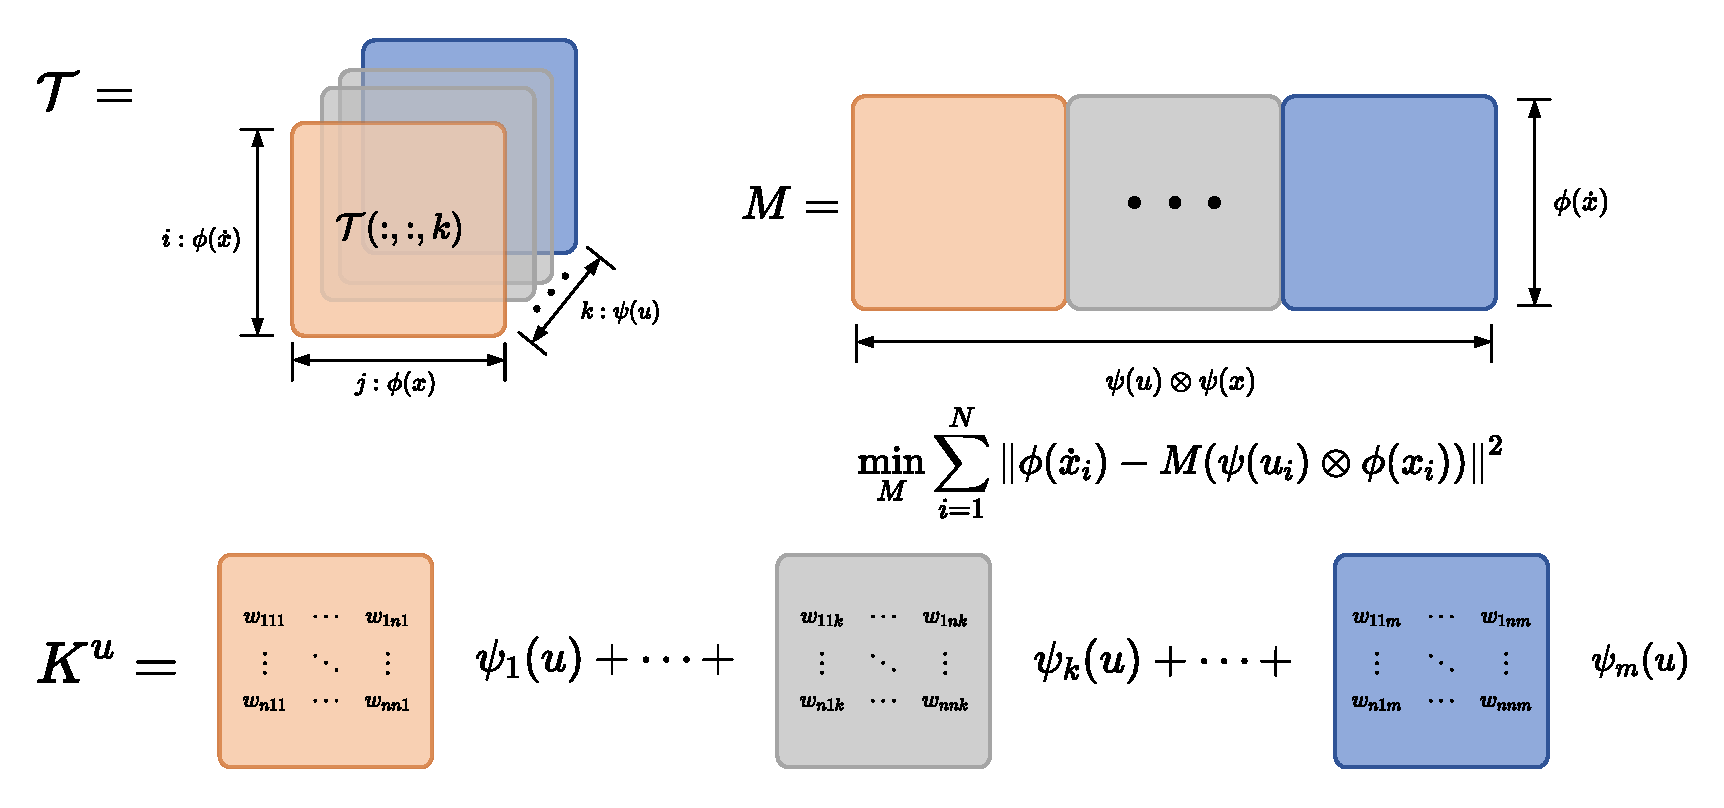
\includegraphics[width=0.95\textwidth]{KUM.pdf}
  \caption{Koopman张量估计}
  \label{KUM}
\end{figure}
我们可以重写上述目标,使其成为一个规则的多变量线性回归问题,
将$\mathcal{T}_K$重新排列为一个大小为$\mathbb{R}^{d_x \times d_x d_u}$的二维矩阵。
令$M \in \mathbb{R}^{d_x \times d_x d_u}$,其中$M[i,:] \in \mathbb{R}^{d_x \cdot d_u}$
是堆叠二维矩阵$\mathcal{T}_K[i, :, :]$所得到的向量,如图[\ref{KUM}]所示。
令$\psi(u) \circledtimes \phi(x) \in \mathbb{R}^{d_x d_u}$为克罗内克积(Kronecker Product),所以有:
\begin{equation}
  K^u \phi(x) = M(\psi(u) \circledtimes \phi(x))
\end{equation}
从而,优化问题变成了常规的线性规划问题:
\begin{equation}
  \min_{M} \sum_{i = 1}^{N} || M(\phi(u) \circledtimes \phi(x_i)) - \phi(\dot x_i) ||^2
  \label{solve_M}
\end{equation}
算法见算法 \ref{KoopmanT} 。

只要我们计算出了$M$,我们就可以通过将$M$转换回为三维张量$\mathcal{T}_K$的方式
为任意系统执行的$u \in \mathcal{U}$得到标准的Koopman算子,
同时也得到了上述对$\mathcal{K}^u$的有限维近似$K^u \in \mathbb{R}^{d_x \times d_x}$

\begin{algorithm}[htbp]
  \caption{Koopman张量估计}
  \label{KoopmanT}
  \begin{algorithmic}[1]
    \Require 状态特征映射 $\phi : \chi \mapsto \mathbb{R}^{d_x}$,
    控制特征映射$\psi : \mathcal{U} \mapsto \mathbb{R}^{d_u}$
    以及一个样本集合:$\{(x_i, u_i)\}_{i = 0}^{N}$
    \State 从等式(\ref{solve_M})中解出$\hat{M}$
    \State 以Fortran风格将$M$转换成$\mathcal{T}_K$
  \end{algorithmic}
\end{algorithm}


\section{最大熵强化学习最优控制问题}
考虑强化学习在最优控制领域的应用,在实践中最大的问题有以下两点:
首先,非常高的样本复杂度:使得智能体在探索中遇到困难;
其次,缓慢、不稳定的收敛过程:探索和利用的权衡是策略优化的重点,
特别是在最优控制中,不合适的样本利用和探索会使得策略过早的收敛到不良的局部最优值。
本文中使用最大熵强化学习算法,通过在训练目标中合理加入熵正则化项。
经过训练,策略可以最大化预期回报和熵。

\subsection{熵正则策略优化}
粗略的说,熵是一个表示随机变量随机程度的量。
具体地说,如果一个随机变量的概率分布很集中,那么这个随机变量的熵就低;
如果一个随机变量的概率分布比较分散,那么这个随机变量的熵就高。

令$x$是具有概率质量密度函数的随机变量$P$。$H$的熵是根据$x$的分布得出的:
\begin{equation*}
  H(P) = \mathop{\mathbb{E}}_{x \sim P} \left[ - \log P(x) \right]
\end{equation*}
在熵正则强化学习中,代理在每个时间步获得与该时间步的策略熵成比例的奖金。
由此,目标策略\cite{haarnoja_reinforcement_2017}变为:
\begin{equation}
  \pi^* = \arg \max_{\pi} \mathop{\mathbb{E}}_{\tau\sim\pi} 
  \left[ \sum_{t = 0}^{\infty} \gamma^t \left( r(s_t, a_t, s_{t + 1}) 
  + \alpha H(\pi(\cdot | s_t) \right) \right]
\end{equation}
其中$\alpha > 0$是权衡参数。我们现在可以在如上假定中给出略有不同的价值函数。
$V^{\pi}$更改为包含每个时间步的熵奖励:
\begin{equation}
  V^\pi = \mathop{\mathbb{E}}\limits_{\tau\sim\pi} 
  \left[ \sum_{t = 0}^{\infty} \gamma^t \left( r(s_t, a_t, s_{t + 1}) 
  + \alpha H(\pi(\cdot | s_t) \right) \left| \right. s_0 = s \right]
\end{equation}
$Q^\pi$更改为包括除了第一个时间步以外的每个时间步的熵奖励:
\begin{equation}
  Q^\pi(s, a) = \mathop{\mathbb{E}}_{\tau \sim \pi} \left[ \sum_{t = 0}^{\infty} \gamma^t
  r(s_t, a_t, s_{t + 1}) + \alpha \sum_{t = 1}^{\infty} \gamma^t H(\pi(\cdot | s_t))
  \left|\right. s_0 = s, a_0 = a \right]
\end{equation}
通过这些定义,$V^\pi$和$Q^\pi$通过以下方程联系起来:
\begin{equation}
  \begin{aligned}
    V^\pi(s) &= \mathop{\mathbb{E}}_{\dot s \sim P, \dot a \sim \pi}
    \left[ r(s, a, \dot s) + \gamma(Q^\pi(\dot s, \dot a) + 
    \alpha H(\pi(\cdot | \dot s))) \right] \\
    &= \mathop{\mathbb{E}}_{\dot s \sim P}
    \left[ r(s, a, \dot s) + \gamma V^\pi(\dot s) \right]
  \end{aligned}
\end{equation}

标准的强化学习最大化奖励之和的期望,但是在加入熵正则方法的强化学习中,
将会考虑一个更加一般的最大熵目标[cite]:
\begin{equation}
  J(\pi) = \sum_{t = 0}^T \mathop{\mathbb{E}} \left[ r(s_t, a_t) 
  + \alpha \mathcal{H}(\pi(\cdot | s_t)) \right]
  \label{MEB}
\end{equation}
权重参数$\alpha$决定了熵项对于奖励的相对重要性,从而控制了最优策略迭代中的的随机性。

\subsection{Soft Actor-Critic强化学习最优控制算法}
下面,介绍如何通过策略迭代公式设计SAC算法\cite{haarnoja_soft_2018},
我们将从推导熵策略迭代(Soft Policy Iteration)开始,
这是一种在应用了熵正则的方法下学习最优策略的通用算法,
在最大熵框架中交替进行策略评估和策略改进。

在策略评估步骤中,我们希望
根据等式(\ref{MEB})中的最大熵目标计算策略$\pi$的值。
对于固定策略,可以从任何函数
$\mathcal{Q} : \mathcal{S} \times \mathcal{A} \mapsto \mathbb{R}$
开始,并且使用下面的修改过的贝尔曼方程迭代计算熵动作价值:
\begin{equation}
  Q(s_t, a_t) = r(s_t, a_t) + \gamma 
  \mathbb{E}_{s_{t + 1} \sim p} \left[ V(s_{t + 1}) \right]
\end{equation}

在策略改进步骤中,策略将逼近于新的熵动作价值函数的指数。
如下的这种特定的设定可以保证策略的改进\cite{haarnoja_soft_2018, sharma_introduction_1998}:
\begin{equation}
  \pi_{new} = \arg \min_{\pi^\prime \in \Pi} \mathrm{D}_{KL} 
  \left( \pi^\prime(\cdot | s_t) \bigg\Arrowvert
  \frac{\exp(Q^{\pi_{old}}(s_t, \cdot)}{Z^{\pi_{old}(s_t)}} \right)
  \label{pi_upd}
\end{equation}

尽管该算法将可证明地找到最优解,但我们只能在表格情况(有限个状态和动作)下以其精确形式执行它。
因此,我们接下来将对连续域进行估计,
其中我们需要依靠函数逼近器来表示动作价值函数,
这种近似的做法产生了一种新的实用算法,称为Soft Actor-Critic算法。

如上所述,大型连续域要求我们推导出熵策略迭代的实际逼近。
为此,我们将对动作价值函数和策略使用函数逼近器,
并且交替使用随机梯度下降(Stochastic Gradient Descent)来优化这两个网络。
我们将考虑参数化状态价值函数$V_\psi(s_t)$、
熵动作价值函数$Q_\theta(s_t,a_t)$
和策略$\pi_{\phi}(a_t|s_t)$。
这些网络的参数是$ \psi, \theta$和$\phi$。
下面介绍这些参数向量的更新规则。

设定如下熵状态函数训练目标,以最小化平方残差:
\begin{equation}
  J_{V}(\psi) = \mathop{\mathbb{E}}_{s_t \sim D}
  \left[ \frac12 ( V_{\psi}(s_t) - \mathbb{E}_{a_t \sim \pi_{\phi}}
  \left[ Q_\theta(s_t, a_t) - \log \pi_{\phi}(a_t, | s_t) \right] )^2 \right]
  \label{v_J}
\end{equation}
其中,$D$是先前采样状态和动作的概率分布,或者是经验回放。
等式(\ref{v_J})的梯度可以用下面的无偏估计表示:
\begin{equation}
  \hat{\nabla} J_V(\psi) = \nabla_\phi V_\phi(s_t) 
  (V_\phi(s_t) - Q_\theta(s_t, a_t) + \log \pi_{\phi} (a_t | s_t))
\end{equation}
其中,动作是根据当前策略采样的,而不是从经验回放中抽取。
可以如下训练熵动作价值函数参数来最小化熵贝尔曼残差:
\begin{equation}
  J_Q(\theta) = \mathbb{E}_{(s_t, a_t) \sim D} \left[ 
  \frac12 (Q_\theta(s_t, a_t) - \hat{Q}(s_t, a_t))^2 \right]
\end{equation}
其中
\begin{equation}
  \hat{Q}(s_t, a_t) = r(s_t, a_t) + \gamma 
  \mathbb{E}_{s_{t + 1 \sim p}} \left[ V_{\overline{\psi}}(s_{t + 1}) \right]
\end{equation}
同样可以用随机梯度下降优化:
\begin{equation}
  \hat{\nabla}_\theta J_Q(\theta) = \nabla_\theta Q_\theta(a_t, s_t)
  (Q_\theta(s_t, a_t) - r(s_t, a_t) - \gamma V_{\overline{\phi}}(s_{t + 1}))
\end{equation}
更新利用了目标值网络$V_{\overline{\psi}}$,其中$\overline{\psi}$
在更新参数时加权更新,
这种方式已可以被证明稳定训练[cite]。
最后,可以通过直接最小化等式(\ref{pi_upd})
中的KL散度(Kullback-Leibler Divergence)来学习策略参数:
\begin{equation}
  J_\pi(\phi) = \mathbb{E}_{s_t \sim D} \left[ D_{KL} 
  \left( \pi_{\phi}(\cdot | s_t) \bigg\Arrowvert 
  \frac{\exp (Q_\theta(s_t, \cdot)}{Z_{\theta}(s_t)} \right) \right]
  \label{Q_J}
\end{equation}
首先使用神经网络变换来参数化策略:
\begin{equation}
  \mathbf{a}_t = f_{\phi}(\epsilon_t;\mathbf{s}_t)
\end{equation}
其中t是输入噪声向量,从一些固定分布中采样,例如球面高斯。我们现在可以将等式(\ref{Q_J})中的目标重写为:
\begin{equation}
  J_\pi(\phi) = \mathbb{E}_{s_t \sim D, \epsilon_t \sim N} 
  \left[ \log \pi_\phi(f_{\phi}(\epsilon_t;s_t) | s_t)
  - Q_\theta(s_t, f_\phi(\epsilon_t;s_t)) \right]
  \label{phi_J}
\end{equation}
我们可以近似等式(\ref{phi_J})的梯度:
\begin{equation}
  \hat{\nabla}_\phi J_\pi(\phi) = \nabla_\phi \log\pi_\phi(\mathbf{a}_t | \mathbf{s}_t)
  + (\nabla_{\mathbf{a}_t} \log \pi_\phi(\mathbf{a}_t | \mathbf{s}_t) - 
  \nabla_{\mathbf{a_t}}Q(\mathbf{s}_t, \mathbf{a}_t)) 
  \nabla_\phi f_\phi(\epsilon_t;\mathbf{s}_t)
\end{equation}
其中,$a_t$由$f_\phi(\epsilon_t;\mathbf{s}_t)$评估。
% 这个无偏梯度估计器将DDPG风格的策略梯度
% 拓展到任何可处理的随机策略。

完整的算法见算法 \textbf{\ref{sac}} 。

\begin{algorithm}[H]
  \caption{Soft Actor-Critic强化学习算法}
  \label{sac}
  \begin{algorithmic}[1]
    \State 初始化参数向量$\psi, \overline{\psi},\theta,\phi$
    \For {每一次迭代}
      \For {每一个时间步}
	\State $\mathbf{a}_t \sim \pi_\phi(\mathbf{a}_t | \mathbf{s}_t)$
	\State $\mathbf{s}_{t + 1} \sim p(\mathbf{s}_{t + 1} | \mathbf{s}_t, \mathbf{a}_t)$
	\State $D \leftarrow D \cup { (\mathbf{s}_t, \mathbf{a}_t, r(\mathbf{s}_t, \mathbf{a}_t), \mathbf{s}_{t + 1}) }$
      \EndFor
      \For {每一次梯度}
	\State $\psi \leftarrow \psi - \lambda_V \hat{\nabla}_\phi J_V(\psi)$
	\State $\theta_i \leftarrow \theta_i - \lambda_Q \hat{\nabla}_{\theta_i}
	J_Q(\phi)$ for $i \in {1, 2}$
	\State $\phi \leftarrow \phi - \lambda_\pi \hat{\nabla}_\phi J_\pi(\phi)$
	\State $\overline{\psi} \leftarrow \tau \psi + (1 - \tau) \overline{\psi}$
      \EndFor
    \EndFor
  \end{algorithmic}
\end{algorithm}

\begin{figure}[htbp]
  \centering
    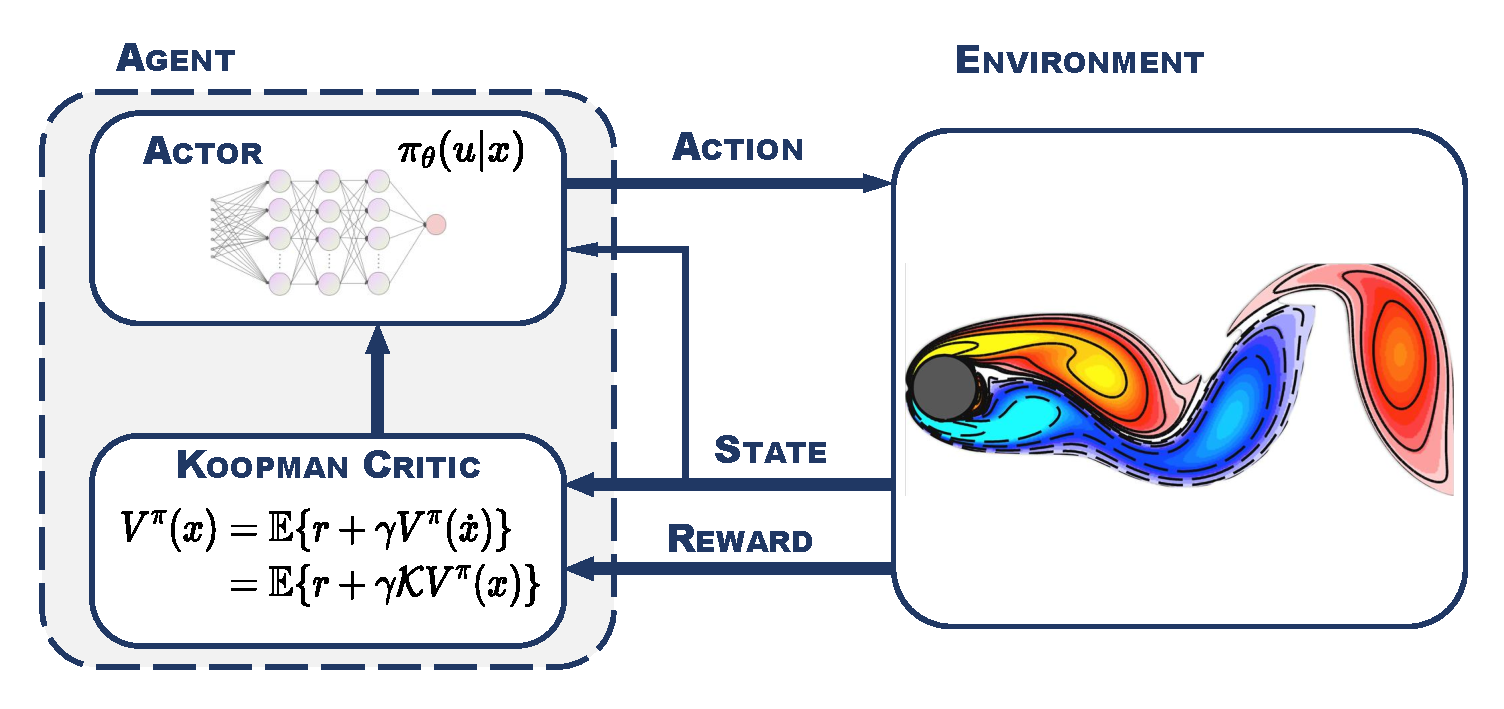
\includegraphics[width=0.95\textwidth]{figures/sakc.pdf}
  \caption{Soft Actor Koopman-Critic}
  \label{fig_sakc}
\end{figure}

下面,介绍如何通过修改Soft Actor-Critic框架[cite],
以合并来自Koopman算子的信息来限制探索空间的。

这里使用与Soft Actor-Critic论文[53]相同的损失函数和类似的符号,
我们首先指定熵价值函数损失:
\begin{equation}
  J_{V}(\psi) = \mathop{\mathbb{E}}_{s_t \sim D}
  \left[ \frac12 ( V_{\psi}(s_t) - \mathbb{E}_{a_t \sim \pi_{\phi}}
  \left[ Q_\theta(s_t, a_t) - \log \pi_{\phi}(a_t, | s_t) \right] )^2 \right]
  % \label{v_J_K}
\end{equation}

在这里,介绍有关Koopman熵价值函数的新定义:
\begin{equation}
  V_\psi(x) = \psi^T \phi(x)
\end{equation}
其中,$\omega$是字典函数的系数向量,表示价值函数在是字典函数也就是观测函数的线性组合。
也就是说,价值函数的评估是集中在Koopman升维后的观测空间中进行的。
同时,我们知道,合理的观测空间应该是由一组完备的观测函数所构建的,
所以在价值评估的准确性上是有理论支撑的。

下面,介绍如何改动动作价值函数的目标函数:
\begin{equation}
  J_Q(\theta) = \mathbb{E}_{(x, u) \sim D} \left[ \frac12 \left( 
  Q_\theta(x, u) - \hat{Q}(x, u) \right)^2 \right]
\end{equation}
其中,训练目标融合了Koopman算子,被定义为:
\begin{equation}
  \hat{Q}(s_t, a_t) = r(s_t, a_t) + 
  \gamma \mathbb{E}_{s_{t + 1} \sim p(\cdot | s_t, a_t)}
  \left[ V_{\overline{\omega}}(s_{t + 1}) \right]
  \label{Koopman-critic}
\end{equation}
在这里,考虑价值预测向量$\overline{\omega}$
和Koopman算子,将上式记为:
\begin{equation}
  \hat{Q}(s_t, a_t) = r(s_t, a_t) +
  \gamma \overline{\omega}^T K^u \phi(s_t)
\end{equation}

最后,策略目标函数并没有更改:
\begin{equation}
  J_\pi(\nu) = \mathbb{E}_{s \sim D}
  \left[ D_{KL}\left( \pi_{\nu}(\cdot | s)
  \bigg\Arrowvert
  \frac{\exp(Q_\theta(s, \cdot))}
  {Z_\theta(s)} \right) \right]
\end{equation}

通过上述修改,实际算法在表述上与算法 \ref{sac}一致。
而不同之处已经在上述公式中解释清楚了。


Koopman辅助的最大熵强化学习以Soft Actor Koopman-Critic为例,
创建了Koopman Critic,其本质是流行的Soft Actor-Critic算法的Koopman变体。

Koopman Critic接收状态和奖励作为原始的非线性动态,然后将这些动态提升到向量空间,
在那个空间里,系统状态可以通过Koopman算子线性地推进。然后将此批评反馈给Actor,
Actor据此计算要在环境中执行的动作。整体的框架如图 \ref{fig_sakc}所示。


\section{本章小结}
本章主要介绍一种用于非线性系统最优控制系统的,基于Koopman算子辅助强化学习训练的算法。
该算法的研究对象主要是第二章中提及的受控非线性系统,训练算法为最大熵强化学习。

同时,通过Koopman算子理论,将最大熵强化学习中的价值函数,
在贝尔曼方程中进行代换的方式,
得到贝尔曼方程中价值函数有关时间序列的期望,
这样做的好处是提高算法对于非线性系统的适应性,
同时保留了Koopman算子对于非线性系统动态的洞察,保留了输入输出的可解释性。


\chapter{深度Koopman算子网络非线性系统最大熵强化学习}
在本章中,首先介绍一个端到端的神经网络学习框架,
用于替代上文介绍的其他数据驱动的Koopman算子,
由于该神经网络架构额外的对于高维度系统动力学信息更好地把握,
可以期望其得到更精准的预测。
同时,将其与Koopman辅助的强化学习结合,得益于更加精确的价值函数估计,
可以使得最大熵强化学习效果更好,训练更快。

\section{深度Koopman算子}
\subsection{深度嵌入函数}
我们首先将嵌入函数分为两部分:
在不失一般性的情况下,我们假设第一项仅与系统状态相关,
$\left.g(x, u)=\left[g_{x}(x, u) ; g_{u}(x, u)\right)\right]$
所以我们得到$g_x(x, u) = g_x(x)$。
基于Koopman算子的定义,将Koopman算子$\mathcal{K}$拆分成两个矩阵,
则可以得出:
\begin{equation}
  g_{x}\left(x_{k+1}\right)=K_{x x} g_{x}\left(x_{k}\right)+
  K_{x u} g_{u}\left(x_{k}, u_{k}\right)
\end{equation}

对于嵌入函数的第一部分,我们使用神经网络$\theta$来参数化$g_x(x, k)$,
将原始状态和网络编码连接起来在一起:
\begin{equation}
  z_{k}=g_{x}\left(x_{k}\right)=
  \left[\begin{array}{c}
  x_{k} \\
  g_{\theta}\left(x_{k}\right)
  \end{array}\right]
\end{equation}
其中$z_k$是升维系统(这里也叫嵌入空间)状态,
$g_\theta : \mathbb{R}^n \mapsto \mathbb{d}$是参数神经网络。
这种设计的优点是可以通过以下方式轻松恢复原始状态:
\begin{equation}
  x_k = C z_k
\end{equation}
其中,矩阵$C \in \mathbb{R}^{n \times (n + d)}$的一个样板如下:
\begin{equation}
  C = \left[ I_n \quad 0 \right]
\end{equation}
这样,我们就可以保留成本函数的形式进行进一步的控制。

对于嵌入函数的第二部分,在深度Koopman算子理论中,
有三个版本来表示$g_u(x_k, u_k)$。

第一个版本被称为深度KoopmanU(Deep KoopmanU with Control, DKUC)算法。
其将函数简化为$g_u(x_k, u_k) = u_k$,
然后演化方程退化为$g_x(x_{k + 1}) = K_{x x} g_x(x_k) + K_{xu} u_k$。

第二个版本被称为深度Koopman仿射
(Deep Koopman Affine with Control, DKAC)算法,
它将进化函数视为控制仿射形式,
使得$g_u(x_k, u_k) = g_u(x_k)u$,
并且将等式 (\ref{Linear_Predictor_K}) 修改为:
\begin{equation}
  z_{k + 1} = K_{x x} z_k + K_{x u} g_u(x_k) u
\end{equation}

对于最终版本,使用控制网络$\phi$将函数$g_u(x_k, u_k)$直接近似为
$g_u(x_k, u_k)=g_{\phi}(x_k, u_k)$,
并且演化函数保持与等式 (\ref{Linear_Predictor_K}) 相同的形式。
它被称为深度Koopman非线性(Deep Koopman Nonlinear, DKN)算法。

给定当前状态$x_t$,我们可以很容易地通过前馈网络预测未来的$K$步状态。
除了嵌入函数外,我们还通过一层线性网络将Koopman
算子矩阵$K_{x x}$和$K_{x u}$参数化,即令$K_{x x}, K_{x u} = B$。
然后K步预测如下:

\begin{equation}
  \begin{array}{c}
    z_{t+k+1}=A z_{t+k}+B g_{\phi}\left(x_{t+k}, u_{t+k}\right), k=0, \ldots, K-1 \\
    z_{t}=g_{x}\left(x_{t}\right)=\left[\begin{array}{c}
    x_{t} \\
    g_{\theta}\left(x_{t}\right)
    \end{array}\right] \\
    x_{t+k}=C z_{t+k}
  \end{array}
  \label{K-steps}
\end{equation}
其中,对于DKUC算法,$g_\phi(x, u)=u$,
对于DKAC算法,$g_\phi(x, u)=g_\phi(x)u$,
对于DKN算法,$g_\phi(x, u)= g_\phi(x, u)$。
网络示意如图 (\ref{control_net})
\begin{figure}
  \centering
  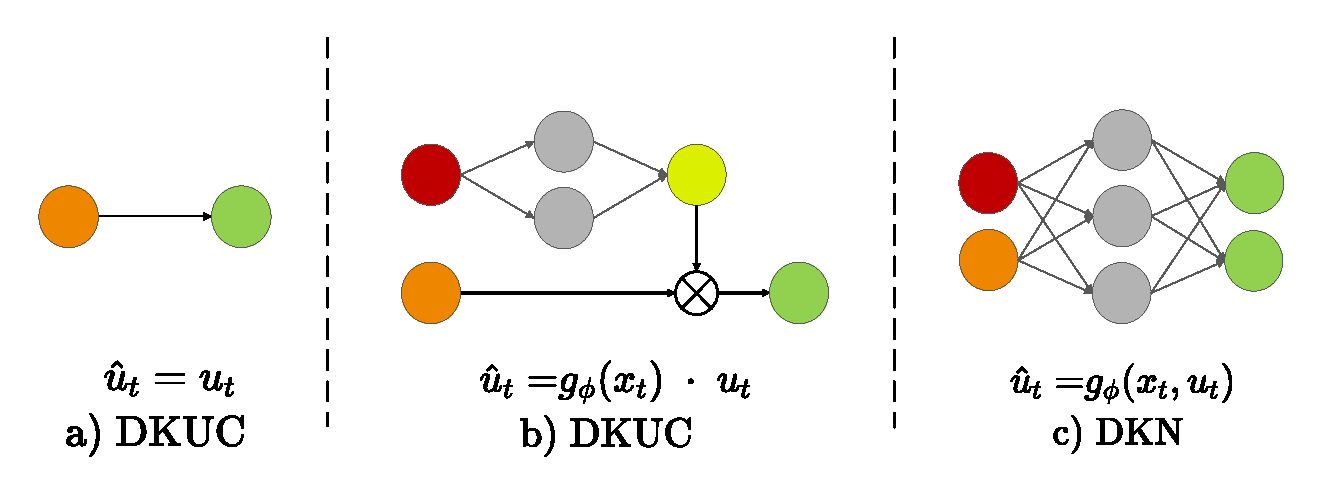
\includegraphics[width=0.95\textwidth]{figures/control_net.pdf}
  \caption{不同形式的控制网络示意图}
  \label{control_net}
\end{figure}

\subsection{K步损失函数}
Koopman的标准算法应首先选择嵌入函数,然后使用线性回归学习Koopman算子矩阵,这种方法仅用于单步预测。
在这项工作中,我们端到端地学习嵌入函数和Koopman算子,并设计了用于长期预测的K步预测损失函数。
给定数据集
$[ X_i \in \mathbb{R}^{N \times n}, U_i \in \mathbb{R}^{N \times m}, i = 0, 1, 2, \cdots, K]$
我们可以计算实际嵌入状态$Z_i = g_x(X)$,
并通过方程 (\ref{K-steps}) 从初始状态$X_0$预测嵌入空间中的K阶状态$[ \hat{Z}_i, i = 1, 2, \cdots, K]$。
损失函数计算如下:
\begin{equation}
  L(\theta, \phi)=\sum_{i=1}^{K} \gamma^{i-1} 
  \operatorname{MSE}\left(Z_{i}, \hat{Z}_{i}\right)
\end{equation}
其中γ是权重衰减超参数,$\operatorname{MSE}$是均方损失函数(Mean Square Error)。
K步损失不是只考虑下面的一步预测误差,而是关注K步预测误差的加权和,
有利于在长时间范围内进行预测。

\section{非线性系统最大熵强化学习}
上一节介绍了深度Koopman算子是如何通过网络架构和而在这一节中,
我们介绍如何将深度Koopman算子和最大熵强化学习结合,
以求使得我们的最优控制算法得到更好的收敛速度和训练效果。

在第三章中,介绍了动作加权的Koopman算子,其目的是为了更好的获取
系统动作的信息,不同的动作量信息,在做单步预测时,
应当在Koopman算子中体现出来,以求达到更好的预测能力。

在实际的控制中,动作变量可能与系统的多个变量有着联系,
甚至其中的数学关系不能够用线性关系来描述,
很明显,简单的加权计算并不能够表述这样的关系。
这就会导致动作的轨迹在升维空间或称之为嵌入空间中
会发生偏移和失真。也就简介导致了Koopman价值函数
在这种情况下会发生误差,导致学习过程受影响。

\subsection{深度Koopman Critic}
下面介绍深度Koopman Critic网络来解决上面的问题:

我们假设有嵌入网络$g_\theta : d_x \mapsto d_z$,控制辅助网络$g_\phi$,Koopman算子矩阵$A, B$和恢复矩阵$C$。
下面介绍网络架构和前馈过程:

有系统状态和输入:$(x_t, u_t)$,嵌入网络将系统状态提升到嵌入空间:
\begin{equation}
  z_t = [\; x_t^T \quad g_\theta(x_t)^T \;]^T
\end{equation}

同样的,辅助控制网络将系统控制提升到嵌入空间:
\begin{equation}
  \hat{u_t} = g_\phi(x_t, u_t)
\end{equation}
这里,使用了深度Koopman非线性形式的辅助网络,
使用了当前时刻系统状态$x_t$和系统控制$u_t$作为输入信息,
在使用了神经网络参数化的策略函数的情况下,
保证了可以准确捕捉动作信息与状态信息之间的关系。

下面介绍两个Koopman算子分量矩阵$A, B$:
\begin{equation}
  z_{t + 1} = A z_t + B \hat{u}_t
\end{equation}
可以看出,在这里我们使用了两个Koopman矩阵,并且取两个矩阵的和作为新的升维状态,
同时考虑了状态信息和动作信息。
具体网络架构如图(\ref{DKN_critic})所示。

在此基础上,我们考虑如等式(\ref{Koopman-critic})中的 Koopman-Critic函数,
将Koopman算子和嵌入函数结合的函数$K^u \phi(\cdot)$通过上述的神经网络结合,
将等式 (\ref{Koopman-critic}) 改写为:
\begin{equation}
  \hat{Q}(s_t, a_t) = r(s_t, a_t)
  + \gamma \overline{\omega}^T ( A z_t + B \hat{u}_t )
\end{equation}

在上面的修改下,我们依然可以遵从算法 
$\ref{sac}$ 对参数网络进行迭代。

\subsection{实验验证}
在本节中,为测试算法性能,在经典的Lorenz环境中进行测试,
这是一个标准的正则混沌基准动力学系统,
由于其连续的特征值谱\cite{brunton_chaos_2017},
通常用于评估基于Koopman的方法。
连续时间动力学由以下方程组给出:
\begin{equation}
  f(x, u)=\left[\begin{array}{c}
  \sigma\left(x_{1}-x_{0}\right)+u \\
  \left(\rho-x_{2}\right) x_{0}-x_{1} \\
  x_{0} x_{1}-\beta x_{2}
  \end{array}\right]
\end{equation}
其中,$\sigma = 10,\ \rho = 28,\ \beta = 8/3$。

文中用了包括SAC、PPO和LQR在内的三种算法
和本章中提出的DSAKC算法作对比。
代码基于CleanRL\cite{huang2022cleanrl}进行改进,实现上述算法在Lorenz环境下的学习。
首先,我让四种算法在Lorenz环境中探索并优化了
$50000$步,并记录下每$2000$步的回报,如图\ref{episodic_return}所示。

\begin{figure}[htbp]
  \centering
  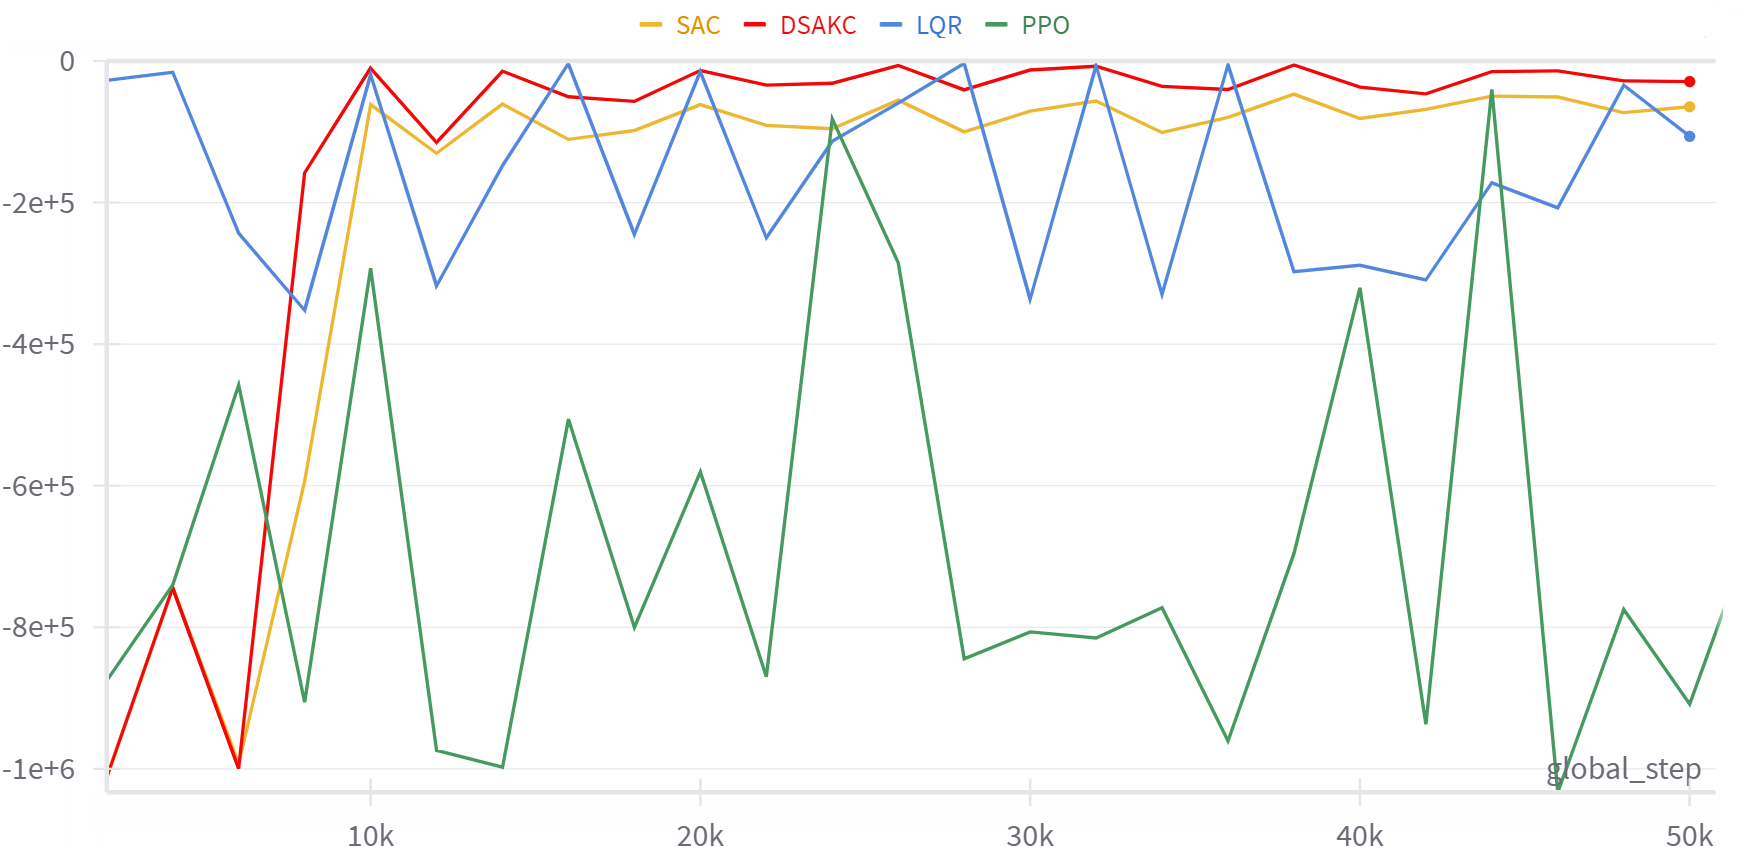
\includegraphics[width=0.99\textwidth]{figures/train_return.png}
  \caption{四种算法在Lorenz系统中每2000步回报曲线图}
  \label{episodic_return}
\end{figure}

比较DSAKC算法和SAC算法,
算法在同一个随机种子的情况下进行训练,
前4000步随机探索,此后的回报均为策略探索得到,
% 我们可以看到DSAKC所得到的回报均在SAC之上,
我们可以看到对于SAC而言DSAKC在Lorenz系统的控制上,有着明显的优势。
\newpage

\begin{table}[h]
  \centering
  \begin{tabular}{ccccc}
    \toprule
    算法 & PPO & LQR & SAC & DSAKC \\
    \midrule
    2000步回报 & -724204 & -156293 & -74895 & \textbf{-33071} \\
    \bottomrule
  \end{tabular}
  \caption{四种算法在Lorenz系统中运行25回合的平均回报}
  \label{average_return}
\end{table}
而对于其他算法,在探索的过程中,并没有表现出持续很好的效果,
但是在探索的过程中,有一些策略在其回合中得到了较小的回报,
下面我将用四种算法训练出的策略,在同样的Lorenz系统中,使用训练中表现最好的
(即回报最小的策略)运行50000步,
即,25个回合,
同时将得到的平均回报绘制成图表,
如表\ref{average_return}所示。

\chapter{总结与展望}
\section{论文总结}
在本文中,我们采用了深度强化学习中的最大熵强化学习的框架对非线性系统进行控制,
其中,熵正则策略优化可以在训练的过程中,加强策略的探索,平衡数据探索和利用,
在解决过早收敛的问题的同时最大化回报。

进一步的,为了解决非线性系统复杂的动力学给价值评估带来的问题,
加入Koopman算子理论,使用Koopman嵌入函数,将系统动力学嵌入到一个更高维的
线性空间中,并使用Koopman算子推进系统动力学。

在现代Koopman算子理论中,Koopman算子可以使用数据驱动的方式得到,
但是嵌入函数的选取仍然是难以解决的问题,
在非线性系统中,根据状态信息构建的嵌入函数,往往会导致动作信息在嵌入空间中产生畸变。
而深度Koopman算子,以及其采用的端到端的训练框架,为嵌入函数加入非线性形式的控制信息,
可以有效地解决此问题。

最后,我提出深度Koopman算子辅助的最大熵强化学习算法,使用Koopman算子及其嵌入函数,
对贝尔曼方程进行改写,将价值估计提升到嵌入空间进行,
使得价值函数可以在高维空间上线性地推进,以提升价值估计的准确性,
进而提升训练的效果,使得智能体在强非线性系统中有比较好的表现。
实验证明,在具有连续谱的非线性Lorenz系统中,
算法展现了比较好的表现,
在50000步的训练和探索中均优于普通的深度强化学习和线性控制算法的表现。

\section{未来展望}
目前,算法主要的问题有两点:
\begin{enumerate}
  \item 深度Koopman算子和最大熵强化学习,采用先后离线训练的方式进行,
    这样会导致样本数据的浪费问题,且无法实现真正的端到端的训练。
  \item 算法实际意义不强,缺失机械臂控制实验。
\end{enumerate}

未来的发展方向主要在于:
\begin{enumerate}
  \item 深度Koopman算子共用经验回放,解决数据浪费的问题;实现在线训练可能。
  \item 寻求与机械臂结合,发挥应对非线性系统优势,实现控制任务。
\end{enumerate}




%论文后部
\backmatter


%=======%
%引入参考文献文件
%=======%
\bibdatabase{bib/database}%bib文件名称 仅修改bib/ 后部分
\addbibresource{bib/database.bib}
\printbib
% \nocite{*} %显示数据库中有的,但是正文没有引用的文献

\Appendix

\begin{figure}[htbp]
  \centering
  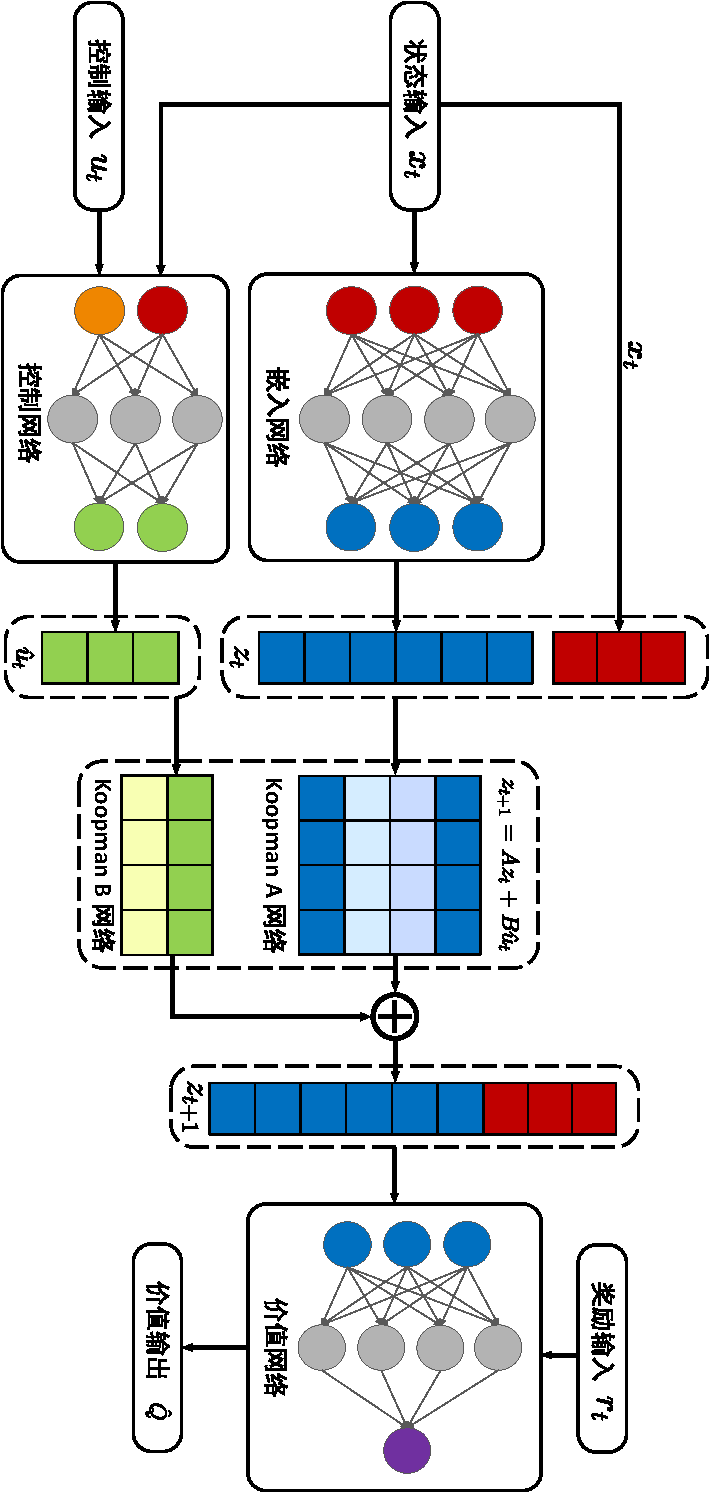
\includegraphics[width=0.52\textwidth]{figures/dkn-rotate.pdf}
  \caption{基于非线性形式辅助网络的深度Koopman价值网络}
  \label{DKN_critic}
\end{figure}

\Thanks

这里是致谢页

\Grade %这一句才是成绩页,上面是填写


\end{document}
